\chapter{Background}

\section{Recommendation Systems}
\subsection{Problem Statement}
Generally speaking recommendation systems are concerned with recommending items to be of use to users.
The recommendations should help the users decide which items to buy, music to listen to, what news articles to read etc.
Virtually any decision-process can be made easier for users by providing recommendations.
Typically recommendation systems are used by online services, famously for example by Spotify for music~\cite{rec_spotify} and YouTube for videos~\cite{rec_yt}.
By using these online service the users generate data that the service can use to improve the recommendations, for example rating videos gives the operator of the service a datapoint on how much a video is liked by a specific user.
However also retailers are known to use recommendation systems, based on data generated by customer loyalty programs such as Migros Cumulus~\cite{rec_migros} retailers tailor coupons or other offers to their customers.
In principle data of users interacting with items (viewing, buying, rating etc.) serves as the basis for a recommendation system. 
Depending on the use-case this data is utilized to assign scores to items depending on the user. 
The semantic meaning of a score depends on the objective of a recommendation system.
For example a system which recommends products to be bought might assign a "probability of purchase", whereas a system which recommends videos might predict the probability of a user watching a video to the end. 
\\
Bringing this all together we can define a general recommendation system with the following function:
\[
    s = f(i, u, h_u)
\]
Where $s$ is the assigned score to item $i$ for the user $u$ and the users history $u_h$. 
The users history represents all the previous interactions with items.
Essentially when we design a recommendation engine we want to learn the function $f$.
To assess the quality of the learned function we need to know the "true" score for the specific item and user, this can be done in different ways.
Usually during training we will hold off later interactions with items, and test the learned functions on those.
However as soon as the users sees recommendations, we essentially change the reality, i.e. we don't know what the user saw as recommendations, if any, in the user history, therefore it makes sense to also assess the performance of a recommendation engine in production.
\subsection{Properties of Recommendation Systems}
In the following we will look at different properties of recommendation systems.
Typically recommendation systems have a combination of the following properties.
\paragraph{User-based}
User-based recommendation system base the information used to make recommendations mainly on properties of the user, such as gender, age, etc.
Also information from the history of the user can be used, for example what the user has bought or read before.
Essentially that means when we try to generate recommendations for a specific user we try to find similar users and recommend items that the similar users liked. 
\paragraph{Item-based}
Item-based recommendation system use mostly information about the item to produce recommendations, such as item type (e.g. genre of a movie).
However as the name suggests, the basis for a recommendation is always a specific item, for example a product a user is looking at online.
This item the user is currently interacting with is referred to as the "active item". 
Usually item-based recommendation systems then try to find similar items to the currently active item. 
The method of finding similar items can be arbitrarily complex, identifying similar items is its own field of research.
What is also often done is combine this approach with a user-based component, where the similar items are sorted or filtered based on the user.
An example of this might be the following:
\begin{itemize}
    \item Steve is a male looking at black shirts.
    \item When extracting similar products we find a range of black shirts, also containing womens shirts.
    \item If we would recommend items by popularity the womens shirts would appear as the first recommendation, since women typically buy more shirts.
    \item Instead of directly displaying the recommendations we filter out the womens shirts that is found in this selection.
\end{itemize}
\paragraph{Session-based}
Session-based recommendation systems are a rather new form of such a system.
A session is a sequence of interactions from a user with one or several items.
Depending on the use-case and setting this can be defined differently.
Usually online-services define a session as the sequence of interactions a user produces on the site until closing the browser window.
Obviously sessions can have variable lengths, therefore it is difficult to directly feed that information into a recommendation system.
However with the rise of Recurrent Neural Networks (c.f.~\ref{rnn}) a powerful tool for handling variable length sequence data becomes available.
Session-based recommendation systems use RNNs to model the sequence data generated by sessions to achieve two things.
First by using RNNs we can extract a fixed dimensional representation of a specific session, this allows us to compare different sessions.
Second by using the fixed representation of a session we can try to identify the intent a user has in a specific session, based on this recommendations can be made to fulfill the users intent.
An intent can be defined as the goal the user has in a specific session.
In the example of an online-shop there are a few different, well-known intents identified by analysts such as: Browsing for inspiration, searching for a specific product, buying a specific product, researching products etc.
Also these intents exist in different contexts, in the case of an online-shop the contexts can be different product types (mobile phone, couch, dining table) etc.
From the above explanation it is intuitive to see why these systems are more desired by operators of online services, since the recommendations can be targeted much more specific to the user and his intent, instead of just general information of the user and the active item. 
\paragraph{Collaborative}
Collaborative recommendation-systems mostly use interaction data to generate recommendations.
For example we use the clicks on products as a data source and then predict which products the user will click next.
However the collaborative aspect comes from the fact that we source other users interactions as a basis for the recommendations.
In principle we view different users as versions of possible behaviour of a user, the more interactions two users have in common, the more similar they are assumed to be.
Therefore we can extend the behaviour (i.e. product views) of a user by looking at what similar users have done on the same active item.
\paragraph{Content-based}
In contrast to collaborative recommendation systems, content-based systems heavily rely on so called content information.
Content information refers to the actual content of different items.
The name stems from early recommendation systems which mainly focussed on recommending media.
The idea is to actually analyze the content of an item, be it the images in a movie, the soundwaves of a song or the text in a book.
The assumption is that a user likes to see items that are similar to each other (e.g. a user who mostly likes action films).
However this method can also be used in different contexts, such as online-shopping, where the "content" of an item might be its textual description or an image of the actual product.
\subsection{Well-Known Examples}
In the following sections we will look at some well-known examples of recommendation engines and their properties.
\subsubsection{Collaborative Filtering via Matrix Factorization}
As the name suggests model is a collaborative approach to a recommendation engine, meaning the model uses primarily interaction data between users and items.
As mentioned in~\cite{intro_recsys} the main idea behind collaborative filtering is to recommend items to the user based on what users with similar taste liked in the past.
Collaborative filtering refers to a class of models that use similar users' tastes to recommend items.
Also this class of models uses the user as a basis for recommendations and not the active item, making it a user-based recommendation system.
As seen in~\cite{collaborative_filtering} there are many ways of implementing a collaborative filtering system.
However the important part is the problem representation.

\begin{figure}[ht]
	\centering
	\captionsetup{width=0.8\textwidth}
    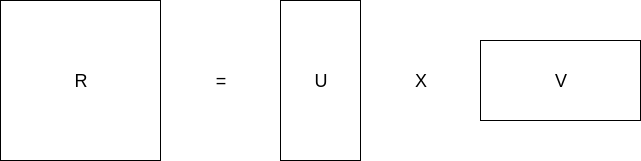
\includegraphics[width=\textwidth]{collaborative_filtering.png}
    \caption{Matrix Completion via Matrix Factorization}
    \label{fig:collaborative_filtering}
\end{figure}
In the Model-Based approach the problem is represented as a matrix completion problem.
The matrix $R$ in figure~\ref{fig:collaborative_filtering} represents the interactions of users and items, where $u_{ij}$ represents the interaction of user $i$ with item $j$.
Usually when dealing with such interaction data, this matrix is very sparse, since in general a user interacts with a small set out of possibly millions of items.
The main idea behind this approach is to fill in the missing entries of the matrix.
To achieve that we define two randomly initialized matrices $U$ and $V$ which when multiplied produce a matrix of the same shape as $U$.
As explained in~\cite{collaborative_filtering} these two matrices represent low rank representations of users and items respectively.
The next step is to use a optimization algorithm to fit $U$ and $V$ such that $r_{ij} \approx UV_{ij}$.
The error of the chosen optimization algorithm however is only applied to entries of $R$ which are known.
Therefore when we find $U$ and $V$ such that the values for the known entries match the values in $R$ we assume that we also found a good approximation for the values unkown in $R$ and use these to predict the interaction of the respective users and items.

\subsubsection{Often Bought Together}
Often/frequently bought together is a recommendation system very popular in online-stores.
The idea behind it is to recommend products that complement the one the user is intending to buy.
A classical example for this would be to recommend a protection case when the users adds a smartphone to the basket.
Therefore it is a item-based approach.
The implementation of this recommendation system can be done in a rather simple way, but can be improved a lot by complex systems, which could personalize the recommendations by using the users history, thereby extending it with a user-based component.
However the basic idea stays the same, as the name suggests, finding items that are frequently bought together.
The simplest, yet still effective, implementation of this is to just count how many times products appear in the same order as other products, i.e. for each combination of two products $i$ and $j$ we will have a count $c_{ij}$ of how many times these products were bought together.
When a user adds a product to the basket, we extract the products with the highest count from a database and recommend these to users.

\section{Concepts}
\subsection{Recurrent Neural Networks}\label{rnn}
Recurrent Neural Networks or RNNs are a form of artificial neural networks, which allow to model sequence input data.
The enabling factor for this is that RNNs allow the output of the network to be fed back in.\todo{Add RNN illustration}.
Further RNNs carry a so called hidden state, which is propagated along the temporal axis.
The following equation describes the general behaviour of a simple RNN.
\[
    
\]
\begin{itemize}
    \item Explain the concept of recurrent neural Networks
    \item What are the problems (vanishing gradients etc)
    \item Explain what a GRU is and why does it handle vanishing gradient better than simple RNN cells?
\end{itemize}
\subsection{Embeddings of categorical data}
\begin{itemize}
    \item What is the problem with categorical data?
    \item What is an embedding, what is the goal?
    \item How can we compute embeddings?
\end{itemize}

\section{Previous Work}
\subsection{Meta-Prod2Vec}
\begin{itemize}
    \item This is a model that allows us to capture the semantic similarity between products
    \item Explain the assumption of word2vec
    \item Show equation of word2vec
    \item How do we apply this to products?
\end{itemize}
\cite{prod2vec}
\subsection{Hierarchical RNNs for personalized Recommendations}
\begin{itemize}
    \item This is the starting point for the thesis
    \item Which components does the system have?
    \item Show the graphic from the paper
\end{itemize}
\cite{hierarchical}

\section{KPIs}
\subsection{Click-Through-Rate}
\subsection{Conversion Rate}\label{conversion_rate}
\begin{itemize}
\item Describe different KPIs
\item What do they meaure, how to optimize for it
\end{itemize}